\documentclass[10pt]{article}
\usepackage[utf8]{inputenc}
\usepackage{graphicx}
\usepackage{amsmath}
\usepackage{hyperref}
\usepackage{amssymb}
\usepackage{geometry}
\usepackage{algorithm}
\usepackage{algorithmic}
\usepackage{verbatim}
\newcommand{\pluseq}{\mathrel{+}=}
\geometry{hmargin=2.2cm,vmargin=2.2cm}
\title{Résolution du problème du labyrinthe par apprentissage par renforcement avec un réseau neuronal - Extraction d'un réseau de neurones des équations de Navier-Stokes}
\begin{document}
\maketitle

Implémentation : \\
\url{https://github.com/Yaaxx/maze-resolution-with-pNS-neurons}


\section{Introduction}
Mon stage s'est déroulé dans l'équipe SequeL à l'INRIA Lille sous la direction de Philippe Preux. L'équipe SequeL s'intéresse à l'apprentissage séquentiel c'est à dire à une forme d'apprentissage où l'information arrive au fur et à mesure que l'agent explore son environnement. Elle travaille notamment sur l'apprentissage par renforcement et sur les problèmes de Bandits.\\
Mon stage est de 6 semaines et je dois travailler sur la résolution du problème du labyrinthe c'est à dire proposer un agent capable de résoudre n'importe quel labyrinthe donné sous la forme de tableau de 0 et de 1. Je dois le faire par apprentissage par renforcement ce qui est un exercice assez classique en utilisant du Q-Learning tabulaire par exemple. Or pour ce stage je vais devoir trouver un moyen de m'affranchir de cette table et utiliser un réseau neuronal à la place. Cette dernière contrainte rend le problème beaucoup plus difficile car les informations sensées être stockées dans la table ne sont pas très continues (à cause des murs qui font une rupture) ce qui rend la table très difficile à remplacer par un réseau de neurones classique tout en conservant de bonnes performances.
L'enjeu de ce remplacement est double : tout d'abord toutes les tables ne peuvent pas être apprisent par Q-Learning ce qui fait que l'utilisation d'un réseau de neurone pourrait être bénéfique car il pourrait être capable de trouver un lien entre ces données. Ceci permettrait alors de pouvoir, avec peu de données, prédire d'autres cases de la table ce qui permettrait d'accélérer fortement la vitesse de résolution d'un labyrinthe par Q-Learning. De plus, ce pouvoir prédictif permettrait une factorisation des informations de la table et donc de réduire l'espace mémoire nécessaire au stockage des informations.\\
Je me suis dans un premier temps intéressé à l'amélioration en temps car de nos jours l'espace mémoire n'est pas vraiment un problème et devoir résoudre un labyrinthe tellement grand que les approches classiques ne fonctionnent plus me semble être un problème qui n'arrive que très peu en pratique. J'ai alors eu une idée assez originale en observant les champs de vecteurs que devait apprendre le réseau neuronal, en effet, ils ressemblaient à un écoulement d'eau dans le labyrinthe. J'ai donc travaillé sur les équations différentielles de mécanique de fluides (Équations de Navier-Stokes) et j'ai cherché à faire un réseau de neurones qui satisferait ces contraintes.\\
Ainsi nous allons tout d'abord voir le contexte scientifique et quelques définition afin de pouvoir suivre cette aventure des équations de Navier Stokes avec des réseaux neuronaux particuliers.

\section{Contexte Scientifique}
\subsection{Apprentissage par renforcement}
L'apprentissage par renforcement est une forme d'apprentissage qui pourrait être vu comme une simulation psychologique du fonctionnement comportemental des êtres vivants. L'agent va devoir maximiser une récompense qu'il va obtenir en effectuant, dans une certaine configuration, une certaine action qu'il aura choisi. Il peut avoir ainsi différentes récompenses, une pour chaque action possible dans la configuration dans laquelle il se trouve et devra maximiser la récompense obtenue (la plupart du temps, sur le long terme). Or l'agent ne connaît pas à l'avance les récompense associées aux différentes actions qui lui sont proposées. Il devra donc les découvrir au fil du temps. Il y a alors un choix à faire : explorer de nouvelles possibilités ou exploiter celles qui sont déjà connues. L'objectif de cet apprentissage est de trouver une bonne politique (fonction de choix, qui a une configuration donnée, donne l'action la plus intéressante) permettant de maximiser la récompense.
\subsection{Q-Learning}
Une des façons de faire de l'apprentissage par renforcement est d'utiliser la méthode de Q-Learning qui consiste en le fait, à partir d'une configuration donnée, de regarder pour chaque action possible les récompenses connues associées. En fonction des données connues et inconnues, on décide d'explorer une nouvelle possibilité ou d'en exploiter une autre. Suite à ce choix, l'agent reçoit de l'environnement la récompense réelle liée à son action qui est alors apprise par l'agent et serra désormais connue. On stocke usuellement ces résultats dans un tableau/dictionnaire et on parle alors de Q-Learning tabulaire.
\subsection{Stratégies simples}
Il existe plusieurs stratégies classiques pour réguler l'exploration et l'exploitation: le epsilon-greedy et le epsilon-first ont l'avantage d'être assez simples. Le concept du epsilon-greedy est de choisir l'exploration avec une probabilité epsilon et d'exploiter le reste du temps (c'est à dire qu'on va beaucoup plus exploiter que explorer). Enfin le epsilon-first consiste en le fait d'explorer pendant les N premiers coups puis d'exploiter le reste du temps. Il existe bien entendu beaucoup de variantes de ces 2 méthodes notamment en faisant varier epsilon en fonction du temps. L'idée étant, la plupart du temps, d'exploiter de plus en plus et donc de faire un mélange bien dosé des 2 concepts.
\subsection{Réseau de neurones}
Un réseau de neurones artificiel est fondamentalement un graphe orienté sans cycle sur lequel va s'effectuer un calcul par propagation de l'information. Certains noeuds sont dits d'entrée et d'autres de sortie. \\
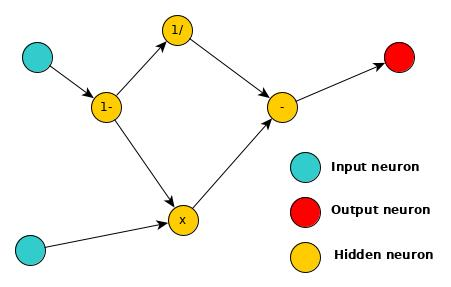
\includegraphics[scale=0.45]{ex_neuron.jpg}\\
Une fois les noeuds d'entrée remplis par une valeur (souvent un réel), le calcul peut commencer : chaque noeud dont toutes les connections entrantes sont déjà calculées peut être calculé à son tour en effectuant l'opération du noeud sur les données entrantes. On peut donc effectuer un calcul par propagation des information des noeuds d'entrée jusqu'à ce que les noeuds de sortie soient tous calculés. On peut alors calculer la fonction représentée par le graphe à partir d'un vecteur d'entrée.\\
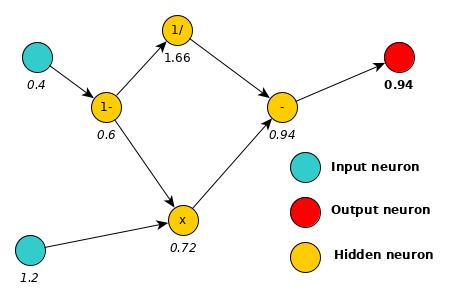
\includegraphics[scale=0.45]{ex_computation_neuron.jpg}\\
Ce qu'on appelle $\textit{réseau neuronal}$ est un tel graphe mais constitué de motifs élémentaires appelés $\textit{neurones}$. Ces neurones sont des petits calculs qui sont, pour les réseaux neuronaux classiques:\\
\indent\indent\indent\indent\indent\indent\indent\indent\indent\indent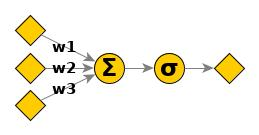
\includegraphics[scale=0.45]{ex_art_neuron.jpg}\\
C'est à dire que l'on somme les entrées pondérées par des wi (appelés poids du réseau de neurones, ce sont des variables internes qui vont servir à l'apprentissage) puis on compose la fonction sigma qui est appelée $\textit{fonction d'activation}$ du neurone. La valeur de sortie est alors envoyé vers l'entrée d'autres neurones formant ainsi un réseau effectuant un calcul. Cette structure imite le fonctionnement des neurones biologiques qui, à partir de potentiels d'action arrivants, et qui sont plus ou moins bien transmis par les synapses, sont sommés puis si le potentiel résultant est suffisant, il se créé un nouveau potentiel d'action au niveau de la $\textit{zone gâchette}$ qui sera transmis aux neurones suivants. Ceci me permet donc d'introduire la fonction d'activation Heaviside qui n'est autre que la fonction indicatrice de $\mathbb{R+}$ (si il y a un signal positif, un potentiel d'action est envoyé). Il existe beaucoup d'autres fonctions d'activation comme relu(x) = max(0,x) qui est très utilisée.\\
Pour faire apprendre un réseau de neurones, la méthode la plus classique est de procéder par descente de gradient : supposons que nous disposons d'un ensemble $(x_i,f(x_i))_{i\in I}$  que nous voulons faire apprendre à notre réseau de neurones. Il va falloir être capable de trouver une fonction dite $\textit{fonction de Loss}$ dépendante de N, la sortie du réseau de neurones, qu'il va falloir minimiser et que cette minimisation permette l'apprentissage efficace de ces paramètres. Une fonction classique est alors la suivante (il en existe plein d'autres):
\[L = \sum_{i\in I}(N(x_i) - f(x_i))^2\]
En effet, cette fonction peut sembler être un bon choix car si L vaut 0, alors on a bien appris tous les points voulus. Pour minimiser cette fonction , on va calculer le gradient de cette fonction de Loss par rapport à chacun des poids du réseau de neurones. On va alors utiliser une règle de mise à jour des poids comme celle-ci : 
\[w_i = w_i-\lambda\frac{\partial L}{\partial wi}\]
Cette méthode permet de "suivre la courbure" de la fonction de Loss et d'adapter les poids de façon à progressivement descendre le gradient de cette fonction. Il faut savoir que le facteur $\lambda\in[0,1]$ est appelé $\textit{facteur d'apprentissage}$ et il permet d'affiner la précision de l'apprentissage : plus il est faible et plus l'ajustement des poids sera précis mais plus il sera lent.\\
Pour calculer ce gradient, de nos jours on utilise une méthode de rétro-propagation dans le réseau de neurones afin de le calculer automatiquement. Il s'agit d'exprimer le gradient de L en fonction des dérivées partielles des valeurs de neurones de sortie. Ensuite on exprime les valeurs des neurones de sortie par rapport à celles des neurones juste avant dans le graphe et on répète ce procédé récursivement jusqu'à ce que on arrive aux entrées (qui sont de dérivée nulle par rapport aux poids car les poids sont entre les neurones et qu'il n'y a plus de neurones avant eux).\\
Ceci est la théorie générale des réseaux de neurones, il faut savoir que la grande majorité du temps les chercheurs préfèrent travailler sur des réseaux de neurones $\textit{par couches}$ (ce ne serra pas notre cas) car cela permet d'avoir des formules de calcul de la sortie avec une expression matricielle ainsi que des formules de descente de gradient plus simples car le réseau est beaucoup plus homogène.\\
\indent\indent\indent\indent\indent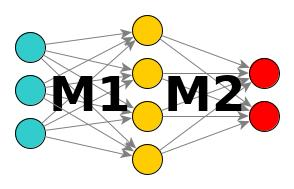
\includegraphics[scale=0.7]{ex_layered_network.jpg}\\

\section{Sujet de Recherche, démarche et résultats}
La méthode dévellopée ci-dessous fonctionne très bien sur le problème précis du labyrinthe. Cependant il faut comprendre que en machine learning on s'interesse à des méthods générales d'apprentissages donc le vrai résultat de ce rapport est la méthode appliquée au problème du labyrinthe et non la résolution du labyrinthe par l'agent. Je vais donc dévelloper dans ces différentes parties les étapes successives du raisonnement ayant permis à partir d'un lot d'équations, de dévelloper un réseau neuronal ayant de comportement voulu.
\subsection{Motivations}
Les approches classiques de résolution du problème du labyrinthe par renforcement avec un réseau de neurones consomment beaucoup plus de place mémoire qu'une approche tabulaire et prennent bien plus de temps pour résoudre le labyrinthe et apprendre une solution \cite{qmaze}. C'est donc le but de mon stage que de trouver une nouvelle approche afin de réussir à mieux utiliser les réseaux de neurones pour résoudre ce problème. 
Après avoir programmé une résolution du labyrinthe par Q-Learning tabulaire, il restait à trouver une forme de réseau de neurones (ce qu'on appelle $\textit{topologie}$ du réseau de neurones) qui serrait capable de remplacer la table. D'après mon maître de stage, il serrait plus simple de trouver une topologie capable d'apprendre les actions à effectuer directement plutôt que les récompenses associées à chaque action. Il s'agirait donc de partir sur une variante du Q-Learning dont le concept serrait, au lieu de stocker une récompense dans la table, de stocker directement les actions les plus rentables pour l'agent. Ceci serrait plus facile à apprendre pour un réseau de neurones. Or si on sait que les réseaux de neurones classiques ne sont pas bons pour résoudre ce problème, je pense qu'il est plus intéressant de partir sur autre chose. En effet, le fait que les réseaux de neurones classiques soient si mauvais à cette tâche n'est pas étonnant, ces approximateurs de fonctions ne peuvent approximer facilement que des fonctions très continues et dès qu'il faut traiter d'un problème peu continu, le nombre de neurones nécessaires explose. Or ce qui fait la puissance des réseaux de neurones est le fait qu'ils soient composés de petits éléments que sont les neurones et que ces neurones vont interagir entre eux dans une structure pour résoudre des problèmes complexes. On peut alors penser que cette difficulté à résoudre ce problème de labyrinthe pourrait venir des composants élémentaires des réseaux de neurones classiques qui sont optimisés pour apprendre des fonctions continues et que en les remplaçant par d'autres mieux optimisés pour les environnements qui ont la forme d'un labyrinthe, on pourrait avoir de meilleurs résultats.\\
 D'un autre coté, en étudiant les tables que le réseau de neurone devait apprendre, j'ai fait le rapprochement avec l'écoulement d'un fluide de l'entrée vers la sortie.

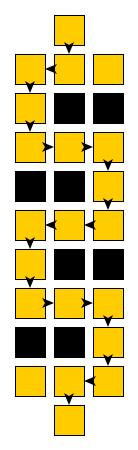
\includegraphics[scale=0.45]{ex_maze.jpg} \indent\indent
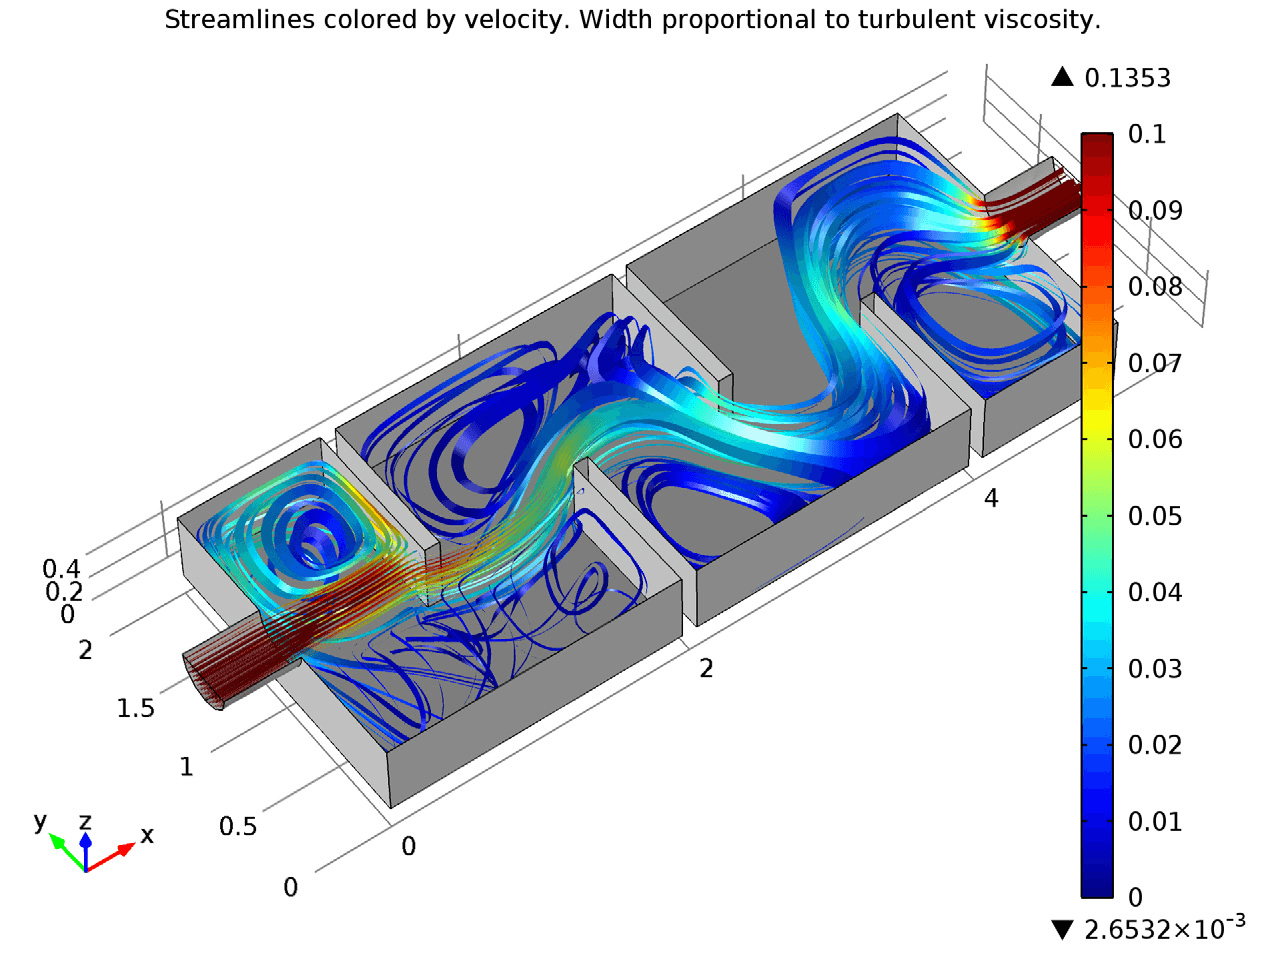
\includegraphics[scale=0.20]{navier.png}\\

Je me suis alors intéressé aux équations de Navier-Stokes qui régissent la mécanique des fluides et je me suis demandé comment il était possible de concevoir un neurone capable d'apprendre efficacement des solutions de ces équations. Puis en me souvenant du cours d'apprentissage d'algorithmique 2 de L3, je me suis dit : "Pourquoi seulement pouvoir approximer facilement des solutions et ne pas plutôt pouvoir apprendre $\textbf{uniquement}$ des solutions ?". Les solutions des équations de Navier-Stokes serraient alors notre ensemble dit d'hypothèses (ensemble des fonctions dans lequel on va chercher notre fonction solution). Il s'agit donc d'une problématique de Deep Learning (faire apprendre efficacement beaucoup de données à un réseau de neurones).

\subsection{Les équations de Navier-Stokes, les contraintes sur les réseaux de neurones}
Les équations de Navier Stokes sur le champs de vitesse sont les suivantes :

\[div \overrightarrow{v} = \overrightarrow{0}\]
\[\rho(\frac{\partial \overrightarrow{v}}{\partial t} + (\overrightarrow{v}.\overrightarrow{\nabla}). \overrightarrow{v}) = -\overrightarrow{\nabla} p + \mu \nabla^2\overrightarrow{v} +\overrightarrow{f}\]

Pour le moment, personne n'a trouvé de solution générale de ces équations différentielles. C'est pourquoi je compte résoudre ces équations numériquement avec un maillage simple : mon labyrinthe est constitué de cases, il s'agirait de prendre un point au centre de chaque case. De plus, ces équations ont une inconnue de plus : le champs de pression $p$. Il va être utile pour coder les murs et la sortie, il s'agira de mettre une plus forte pression dans les murs (environ 100 fois plus que dans les couloirs) ainsi que une pression très très faible à la sortie (environ 10**5 fois moins que dans les couloirs) afin que le flux converge vers cette case. Maintenant que le labyrinthe est modélisé, on va supprimer les termes inutiles des équations : je n'ai pas besoin d'un facteur temporel car les fluctuations temporelles ne m'intéressent pas. On va aussi oublier le terme de viscosité (plutôt utile près des bords mais je ne m'intéresse que au centre des cases) ainsi que le terme de force car on a codé les murs dans le champs de pression. Voici les nouvelles équations de Navier-Stokes que je vais utiliser :

\[div \overrightarrow{v} = \overrightarrow{0}\]
\[\rho (\overrightarrow{v}.\overrightarrow{\nabla}).\overrightarrow{v}  = -\overrightarrow{\nabla} p \]

A partir de ces équations, il va être possible de récupérer quelques résultats théoriques assez intéressants.\\ 
Tout d'abord, on ne sait pas actuellement résoudre ces équations explicitement. Il n'est donc pas question d'essayer même de manière détournée de les résoudre pendant mon stage, il va donc être important de baliser le terrain avant d'essayer de faire quoi que ce soit afin d'espérer trouver quelque chose dans mon court séjour au laboratoire. Je vais donc aller beaucoup plus loin dans ces hypothèses et même supposer qu'elles n'ont pas de solution trouvables avec les outils mathématiques actuels. Ainsi comme la plupart des réseaux de neurones classiques ont une sortie calculable explicitement à partir d'un graphe, si j'arrivais à résoudre mon problème général, alors je pourrais résoudre Navier-Stokes ce qui est exclus. Avec cette simple réduction je sais déjà que je ne pourrais pas résoudre mon problème avec un réseau de neurones 100\% explicite. Il va donc devoir y avoir des noeuds qui vont devoir exécuter des opérations non triviales comme par exemple résoudre des équations dont on ne connaît pas de solution exacte. On pourrait alors se dire "On va soigner le mal par le mal" et essayer de faire un réseau de neurones dont tous les noeuds serraient des résolutions approchées de sous-équations différentielles et que la sortie finale soit une solution approchée des équations de Navier-Stokes. Cette méthode m'a paru assez originale mais n'a rien donné de mon coté (c'est une piste qui peut être très intéressante à suivre mais qui dépasse complètement mes connaissances en équations différentielles actuellement). \\
De plus, si je fais un réseau de neurones, j'ai besoin de le faire apprendre (sinon je ne pourrais jamais le faire remplacer ma table). La méthode d'apprentissage la plus utilisée est la descente de gradient, je dois donc être capable de dériver partiellement mes fonctions dans mon réseau de manière explicite si possible (il faut être précis quand on fait des descentes de gradient). Ces fonctions sur mes noeuds doivent donc être de dérivée explicite mais qu'on ne puisse pas les intégrer explicitement sinon on résoudrait Navier-Stokes. Ce jeu de contraintes était suffisamment complexe pour que je pense à une autre solution.

\subsection{Navier-Stokes par un réseau de neurones, contourner les contraintes}
Si je ne peux pas apprendre par descente de gradient, il va falloir trouver une autre façon d'apprendre. De plus, les équations différentielles sont des équations de continuité locale et mes dérivées sont selon X et Y. L'idée la plus logique serrait alors de faire un plan de neurones, il serrait alors plus simple de faire ces dérivées partielles. De plus, pourquoi ne pas faire dans un premier temps une "table de neurones", on n'y gagnerait pas en place par rapport au Q-Learning tabulaire mais on pourrait utiliser la puissance d'induction des réseaux de neurones pour apprendre les liens qui lient les éléments de la table et donc pour avoir un pouvoir prédictif bien supérieur à la méthode tabulaire. On aurait alors un gros gain en temps. L'intérêt de cette table de neurones serrait aussi d'avoir une méthode d'apprentissage efficace car on n'aurait que a donner au neurone la valeur qu'on veut qu'il apprenne (ce ne serraient plus les connections entre neurones qui auraient des poids mais les neurones eux-mêmes) puis il se chargera de reconstruire une solution de Navier-Stokes en modifiant légèrement les neurones aux alentours en profitant de cette structure de plan pour faire ses calculs efficacement. Ceci semble donc une bonne approche qui contourne les contraintes théoriques précédentes.

\subsection{Résoudre les équations de Navier-Stokes de manière séquentielle}
Maintenant que l'on a une piste de topologie, il m'a semblé important de vérifier que cette solution était bien en accord avec le sujet posé et qu'elle y répondrait bien. Vu que l'on a un agent qui va se déplacer dans le labyrinthe, il est important que cet apprentissage puisse se faire de manière progressive. On va devoir par conséquent trouver une manière de résoudre Navier-Stokes dans ces conditions. Le soucis est que quand on arrive dans un cul de sac, les équations de Navier-Stokes (notamment la divergence), disent que toute la composante doit avoir une vitesse de 0 (eau stagnante car elle n'est pas dans le courant qui relie l'entrée à la sortie). Or si on se permet de faire une propagation de cette information dans les neurones pour la faire remonter et changer ceux de toute l'aile, ce ne serrait pas un coût énorme par rapport à un réseau de neurones classique qui nécessite à chaque apprentissage de rétro-propager de l'information à travers tous ses neurones. Cependant on peut faire mieux : dans tous les cas l'agent devra ressortir de l'impasse donc autant corriger les valeurs de vitesse au fur et à mesure qu'il remonte. De plus dans le cas de croisements, on peut avoir des problèmes :
\indent\indent\indent\indent\indent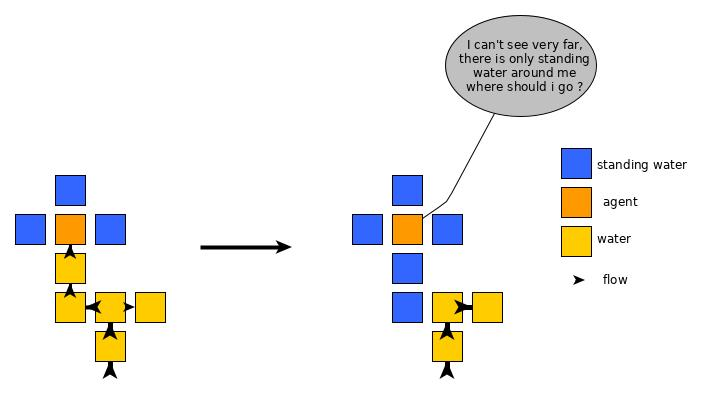
\includegraphics[scale=0.45]{question.jpg}\\
Or si on résolvait de manière séquentielle, on pourrait faire en sorte que l'agent suive la courant au fur et à mesure et le remonte (c'est une optimisation dont je reparlerai plus tard). Il y a cependant un potentiel problème à résoudre la divergence en cas de cycle de manière séquentielle. \\ 
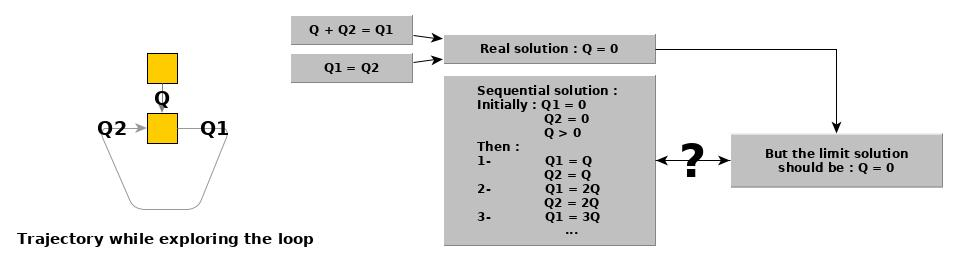
\includegraphics[scale=0.45]{ex_div_diverge.jpg}\\
En effet, en fonction de notre façon de résoudre les équations, les valeurs de vitesse pourraient s'emballer et l'agent pourrait se retrouver bloqué dans la boucle. Il faudra donc bien y réfléchir dans la suite. Enfin, la dernière équation n'est clairement pas triviale donc je vais me contenter de la discrétiser et de voir ce que cela va donner séquentiellement, elle contient toute la complexité des équations de Navier-Stokes et est donc la raison de la plupart des problèmes depuis le début, il faut donc la manipuler avec précaution.

\subsection{Vers des équations plus discrètes}
Après avoir fait une première implémentation d'une résolution de Navier-Stokes, je me suis rendu compte que ces équations se sont vraiment résolubles numériquement que dans des environnement très continus. En effet, une simple imprécision peut avoir des effets énormes sur la suite de la résolution. J'ai alors pensé à essayer d'augmenter la résolution de mon environnement afin d'avoir des solutions moins approchées et plus continues, puis de faire une moyenne sur chaque case mais cela restait assez compliqué notamment vu le nombre d'inconnues dans les équations.
J'ai alors eu l'idée de refaire des équations de "Navier Stokes" adaptées à un environnement plus discret. En voici la liste :
\[ div(\overrightarrow{v}) =
\begin{cases}
	\alpha & \text{à l'entrée} \\
	-\alpha & \text{à la sortie} \\
	0 & \text{sur le reste des cases}
\end{cases}
\] 
\[ \overrightarrow{v} = \overrightarrow{ave}\overrightarrow{v} +\lambda\overrightarrow{v_{learn}} +\overrightarrow{dev}\]

avec, pour la notation suivante :\\
\indent\indent\indent\indent\indent\indent\indent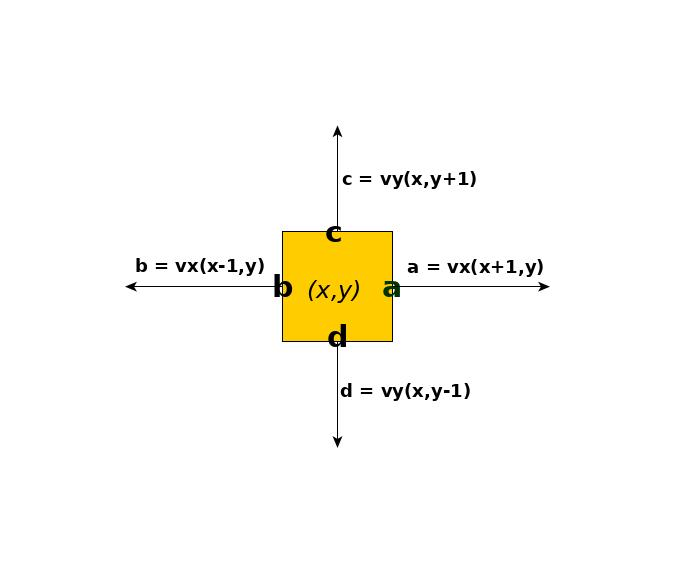
\includegraphics[scale=0.3]{notation.jpg}\\
les expressions suivantes :

\[ \overrightarrow{v} = 
\begin{pmatrix}
vx \\
vy
\end{pmatrix}
\]

\[\overrightarrow{ave}\overrightarrow{v} = 
\begin{pmatrix}
\frac{a+b}{2} \\
\frac{c+d}{2}
\end{pmatrix}
\]

\[\overrightarrow{dev} = \mu.sv(vx.vy).([\mathbf{1}_{\mathbb{R_-^*}}(c.vy)+\mathbf{1}_{\mathbb{R_-^*}}(d.vy)].\frac{\|vy\|}{2}-[\mathbf{1}_{\mathbb{R_-^*}}(a.vx)+\mathbf{1}_{\mathbb{R_-^*}}(b.vx)].\frac{\|vx\|}{2}).
\begin{pmatrix}
1 \\
-1
\end{pmatrix}
\]

\[\mu = \mathbf{1}_{\mathbb{R_+}}(-1+\sum_{\substack{(i,j)\in[-1,0,1]\\i.j=0}}{P(x+i,y+j)})\]

\[ P(x,y) = 
\begin{cases}
	1 & \text{si il y a un obstacle en x y} \\
	0 & \text{sinon}
\end{cases}
\]

\[sv(x) = 
\begin{cases}
	sgn(x) & sgn(x) \neq 0 \\
	random(\{-1,1\}) & sinon
\end{cases}
\]


Le terme de divergence indique simplement une conservation de la matière. Enfin la deuxième équation se compose en 3 termes : un terme de continuité: 
\[\overrightarrow{ave}\overrightarrow{v}\]
un terme d'apprentissage forcé:
\[\lambda\overrightarrow{v_{learn}}\]
et un terme d'exploration :
\[\overrightarrow{dev}\]
Le terme de continuité sert à essayer de conserver une continuité de vitesse entre les cases. Cependant ce terme n'est pas parfait et n'assure pas une conservation de la matière sans failles ce qui posera des problèmes pratiques plus tard (on pourrait ajouter un terme de correction assez facilement mais je voulais rester sur quelque chose de relativement simple). Le terme d'apprentissage forcé permet d'augmenter la valeur de vitesse dans un sens ou dans l'autre en fonction de ce que l'on veut faire. Il est donc plutôt là pour inciter le réseau de neurones à considérer une solution particulière allant plutôt dans une direction à partir d'un point. Enfin le dernier terme permet de faire en sorte que le réseau neuronal explore par lui même (voir chapitre suivant), ce qui rend justement ce facteur d'apprentissage anecdotique. Le plus gros du travail serra fait pas le pouvoir de prédiction du réseau neuronal et ses suggestions d'exploration. On a donc intégré une partie de l'apprentissage par renforcement au réseau neuronal qui saura lui-même quand il a besoin d'explorer.

\subsection{Résolution des équations de "pseudo Navier Stokes"}
Maintenant que nous avons des équations satisfaisantes, il va falloir essayer de les résoudre afin de tirer un réseau neuronal de cette résolution. Le principe de l'apprentissage séquentiel est que nous n'allons regarder que les cases adjacentes à notre agent et résoudre ces équations sur ces cases. Pour qu'elles soient résolues de manière plus pertinente, vu que l'agent est en mouvement, on considère qu'il arrive d'une case adjacente et que l'on veut résoudre les équations sur la nouvelle case sur laquelle il arrive. On suppose donc que la valeur de la case depuis laquelle l'agent vient est correcte, elle serra donc considérée comme étant une constante, ce qui permettra de véritablement propager de l'information dans la labyrinthe. De plus on suppose que la vitesse dans les murs est de 0 (donc constante), ce que l'on peut écrire en modifiant la première équation de la forme (mais elle est un peu moins digeste) :

\[ \sum_{i\in[-1,1]}vx(x+i,y)(1-P(x+i,y))+vy(x,y+i)(1-P(x,y+i)) = 
\begin{cases}
	\alpha & \text{à l'entrée} \\
	-\alpha & \text{à la sortie} \\
	0 & \text{sur le reste des cases}
\end{cases}
\] 

On pourrait aussi garder l'ancienne équation et ajouter celle ci, beaucoup plus digeste mais moins explicite à résoudre :
\[P\overrightarrow{v} = \overrightarrow{0} \]

Ainsi pour résoudre la divergence, si on est dans un couloir, on a 2 murs, et la case de derrière donc il ne reste qu'une inconnue : on peut résoudre. On remarque que si on est dans un cul de sac, on n'a pas d'inconnue et seulement dans ce cas on se permet de modifier la case de derrière (qui vaudra 0 par conséquent). Dans les cas de croisements, il existe plusieurs solutions aux équations de Navier-Stokes et il en est de même pour nos équations de "pseudo Navier Stokes". Il va donc falloir faire un choix pour les résoudre. Pour ce faire, on va faire le choix d'augmenter les courants déjà existants proportionnellement à leur force (un courant faible serra peu affecté tandis qu'un courant fort variera beaucoup plus). On va donc utiliser ces formules :
\[v\alpha(x+a,y+b) \pluseq 
\begin{cases}
	\frac{s.\Delta div.\|v\alpha(x+a,y+b)\|}{somme} & \text{si somme $\neq$ 0 $\rightarrow$ terme d'exploitation et de renforcement} \\
	\frac{s.\Delta div}{nb\_couloirs} & \text{si somme = 0 $\rightarrow$ terme d'exploration équitable}
\end{cases}
\]
avec a et b dans [-1,0,1] tels que a.b = 0 et $\alpha$ pouvant signifier x ou y
\[s = a+b \rightarrow\text{désigne le signe de variation de la grandeur}\]
\[\Delta div = - div(\overrightarrow{v})(x,y) +
\begin{cases}
	\alpha & \text{(x,y) est l'entrée} \\
	-\alpha & \text{(x,y) est la sortie} \\
	0 & \text{sinon}
\end{cases}
\]
\[somme = \sum_{i\in[-1,1]}\|vx(x+i,y)\|(1-P(x+i,y))+\|vy(x,y+i)\|(1-P(x,y+i)) \]
\[nb\_couloirs = \sum_{\substack{(i,j)\in[-1,0,1]\\i.j=0}}{P(x+i,y+j)}\]
Avec ces formules on trouve les nouvelles valeurs des neurones proches en faisant varier a et b (on ne doit pas essayer de résoudre la divergence dans un mur (si (x+a,y+b) est un mur), c'est écrit dans les équations). \\
Maintenant que l'on connaît les valeurs des neurones proches, on va pouvoir trouver la valeur du neurone en (x,y), pour cela il suffit simplement d'utiliser la formule donnée précédemment. Attention cependant, les valeurs de vitesse pour les cases adjacentes qui apparaissent dans le terme de déviation ($\overrightarrow{dev}$) sont celles $\textbf{avant}$ la correction de la divergence (sinon ça marche beaucoup moins bien).
Je vous laisse tester vous même le code sur le github si vous voulez voir comment cela fonctionne (cf résolution par rna simulé).

\subsection{D'une résolution séquentielle sans propagation vers un réseau neuronal}
Le sujet du stage reste de résoudre le problème avec un réseau de neurones. Il va donc falloir s'y ramener mais tout le travail effectué jusqu'à maintenant a été fait pour rendre cette tâche plus facile. En effet, on a une résolution locale des équations (c'est pourquoi les équations différentielles peuvent être intéressantes pour faire des réseaux de neurones en apprentissage séquentiel), ce qui permet de résoudre l'équation sur chaque point en n'interagissant que avec ses voisins (il faut tout de même que ces points soient accédés tours à tours selon une trajectoire car les équations ont étées faites pour un apprentissage séquentiel). On peut donc imaginer un plan avec des motifs élémentaires qui organiseraient leur voisinage immédiat en communiquant entre eux tout en respectant le procédé décrit ci-dessus qui ne donne que des solutions des équations de "pseudo Navier Stokes". J'ai donc construit le graphe de ces calculs afin de dessiner des machines élémentaires qui seront nos neurones.

(cf Annexes)

Ces neurones sont contrairement aux neurones classiques composés de plusieurs $\textit{organites}$ c'est à dire qu'ils ne font pas que de modifier leur valeur puis de la transmettre aux autres mais il peuvent aussi servir d'intermédiaires et prendre des données aux neurones voisins, faire un calcul dessus et leur renvoyer le résultat du calcul sans modifier leur propre valeur.

Nous avons donc bien réussi à faire un réseau de neurones qui ne peut donc apprendre que des solutions des équations de "pseudo Navier Stokes".

\subsection{Lien avec l'apprentissage par renforcement}
Maintenant que nous avons résolu notre problème de Deep-Learning, il va falloir raccorder notre solution à notre algorithme d'apprentissage par renforcement. On peut faire apprendre des valeurs de vitesse au réseau de neurones mais cela sert plus à orienter le flux à travers le labyrinthe que à réellement se souvenir de la valeur exacte des vitesses donnée. Ceci vient du fait que le réseau de neurones à déjà un terme d'exploration incorporé et que ce terme est déjà régulé par le réseau lui-même. Il va donc falloir un peu modifier l'algorithme d'apprentissage par renforcement si on veut avoir de bons résultats. En effet, il va falloir tenir compte de ces capacités d'anticipation et d'exploration du réseau de neurones qui le rendent bien meilleur que la plupart des réseaux de neurones actuels qui se contentent de mémoriser betement. Ces compétences vont se manifester par une proposition de trajectoire immédiate (juste à coté de la case sur laquelle est l'agent) que l'agent pourra suivre ou non. La seule chose que l'agent a à faire est de suivre ce que le réseau de neurone lui indique de faire. On peut cependant si l'on veut ajouter une influence sur cette exploration / exploitation en utilisant le vecteur d'apprentissage forcé afin d'influencer les choix du réseau de neurones. Attention cependant à ne pas donner d'informations erronées (comme foncer dans un mur ou revenir en arriere) avec une norme trop importante sinon cela pourrait créer un bug au niveau de la logique de résolution du réseau de neurones qu'il devra essayer de fixer lui-même. C'est pourquoi il est peu recommandé d'utiliser ce terme d'apprentissage forcé. On peut alors se demander quel est le terme qui fait apprendre le réseau de neurone et c'est la valeur de la divergence de la case qui représente pour l'apprentissage par renforcement la récompense.\\
Il reste à déterminer comment, à partir du réseau neuronal, choisir quelle direction prendre. La façon dont on va choisir la prochaine case sur laquelle aller à partir du réseau de neurones va dépendre non seulement de la case actuelle mais aussi des cases connexes : on détermine un score pour chaque axe : x et y :
\[scorex = 
\begin{cases}
	0 & sgn(x) = 0 \\
	vx(x,y).vx(x+sgn(vx),y) & sinon
\end{cases}
\]

\[scorey = 
\begin{cases}
	0 & sgn(y) = 0 \\
	vx(x,y).vx(x,y+sgn(vy)) & sinon
\end{cases}
\]
Une fois ces grandeurs calculées, on prend la plus grande, ce qui permet de choisir l'axe du mouvement, puis il reste à choisir le sens : on choisit selon le signe de la grandeur choisie. Voici un algorithme qui résume tout ça et qui traite des cas particuliers:
\begin{algorithm}
\caption{Select movement}
\begin{algorithmic}
\STATE $VX \leftarrow vx(x,y)$
\STATE $VY \leftarrow vx(x,y)$
\STATE $scorex \leftarrow vx(x+sgn(VX),y)*VX$
\STATE $scorey \leftarrow vx(x,y+sgn(VY))*VY$
\IF{$abs(scorex) > abs(scorey)$}
\IF{$sgn(scorex) == 1$}
\STATE move(right)
\ELSE 
\STATE move(left)
\ENDIF
\ELSE
\IF{$abs(scorey) == abs(scorex)$ and $scorex == 0$}
\STATE r\_move $\leftarrow$ choose\_a\_random\_possible\_move()
\STATE move(r\_move)
\ELSE
\IF{$sgn(scorey) == 1$}
\STATE move(top)
\ELSE
\STATE move(bottom)
\ENDIF
\ENDIF
\ENDIF
\end{algorithmic}
\end{algorithm}

Ce cas où scorex = scorey = 0 arrive quand l'agent à trouvé une impasse et essaie donc de remonter le cours d'eau pour retrouver du courant. C'est ici que l'on va pouvoir aider le réseau de neurones car il a raison de dire que les vitesses sont nulles mais il ne faut pas que l'agent se perde en cas de croisement (cf partie 3.4). Il suffit donc, avant de résoudre la divergence, de chercher une case de vitesse non nulle à proximité et de s'y déplacer si la valeur de vitesse de la case actuelle est 0. Cette opération se fait en temps et espace constant donc je me suis permis de l'implémenter sur le github. La convergence est ainsi plus rapide.

\subsection{Limites techniques de l'implémentation}
L'implémentation d'un tel algorithme pose plusieurs problèmes technique dont un majeur qui n'affecte pas le fait de trouver une solution mais qui gène en cas d'exploration de structures très arborescentes dans le labyrinthe. En effet, il y a une faille dans les équations que j'ai trouvées (j'en avait déjà parlé dans le chapitre consacré à leur introduction). La conservation de la matière n'est pas respectée parfaitement par la seconde équation. Si rien n'entrait en conflit avec ça, tout fonctionnerait toujours bien (j'avais prévu l'éventualité en concevant les équations, ce n'était pas grave pour la résolution). Or régulièrement, quand l'agent arrive dans un cul de sac, il doit mettre les valeurs de ce couloir à 0. Ce qui fait qu'il calcule le terme vu précédemment pour résoudre l'équation de divergence. Cependant ce terme qui doit être l'opposé de la valeur actuelle sur la case a été calculé différemment de la valeur actuellement sur la case. Il en résulte un problème bien connu des flottants en informatique : on n'obtient pas parfaitement 0. Or l'algorithme fait une très grande différence entre les valeurs valant 0 (pas de courant) et celles ne valant pas 0 ce qui fait qu'il va falloir "cut" ces valeurs trop faibles pour les mettre à 0. J'ai finalement réussis à séléctionner les valeurs à cut de celles qui ne faut pas cut donc ce problème ne se pose plus dans ce sens.

\subsection{Résultats et comparaison au Q-Learning classique}
J'ai comparé la méthode de résolution par les neurones de Navier-Stokes au Q-Learning tabulaire et les résultats sont assez impressionants (cf Annexes). Pour des soucis d'équité, j'ai implémenté quelques améliorations à l'algorithme de Q-Learning : tout d'abord dans un labyrinthe que l'on arrive sur une case depuis le haut, la gauche, la droite ou le bas n'a aucune importance au niveau de la récompense associée. Ainsi au lieu d'associer une récompense à un couple (état, action), je n'ai compté que l'état dedans. De plus, j'ai empéché l'agent de faire demi-tour dans le labyrinthe (j'ai gardé en mémoire sa derniere position et il ne pouvait plus y aller en explorant à moins qu'il n'ait pas d'autres alternatives). Pour faire du Q-Learning tabulaire on utilise la loi de mise à jour de la table suivante (Q étant le tableau des récompenses, r la récompense réelle et move(s,d) la fonction qui a une position s et une direction d associe la nouvelle position s' suite au mouvement):
\[Q[s] \pluseq \alpha(r+\gamma.max_dQ[move(s,d)]-Q[s])\]
avec pour mes calculs : $\alpha$ = 0.3 et $\gamma$=0.92. Une récompense de 1 à l'arrivée et de -0.001 sur toutes les autres cases (afin qu'il trouve le meilleur chemin). L'implémentation est sur le github.
Les courbes analysent les performances des 2 apprentissages sur 3 labyrinthes 25x25 différents générés aléatoirement selon l'algorithme de Wilson. Chaque courbe représente 150 tests d'apprentissages depuis 0 sur 500 résolutions completes de labyrinthes (une résolution est appelée un $\textit{episode}$) et montre le nombre de pas dans le labyrinthe pour le résoudre (en échelle logarithmique). Chaque courbe est affichée avec un paramétre d'opacité de 0.01 ce qui donne une figure de densité afin de voir la fiabilité de chaque méthode.
L'algorithme de Navier-Stokes fonctionne également très bien sur des labyrinthes plus grands : j'ai essayé 100x100 mais je ne peux pas tester sur beaucoup plus grand car l'algorithme de Wilson a une complexité exponentielle. Les 25 000 labyrinthes générés par cet algorithme en prévision du stage sont disponibles sur le github (je n'ai pas pu tous les tester faute de temps et de puissance de calcul, je me suis donc interessé que aux premiers).
On peut noter quelques pics au niveau de la courbe verte après le premier. Ceux-ci sont liés au problème des flottants qui fait que l'agent se perd dans des zones d'eau stagnante.

\subsection{Conséquences de ces travaux}
Ces travaux ont permis de créer un réseau de neurones fait spécifiquement pour les besoins du problème à partir de contraintes sous formes d'équations. Cette méthode diffère de beaucoup des autres méthodes similaires dans le sens où, on n'utilise pas la fonction de loss des réseau de neurones classiques pour approcher des solutions mais on est certain à 100\% que les contraintes sont respectées. Ces contraintes offrent au réseau de neurones un pouvoir prédictif très puissant lui permettant de résoudre le labyrinthe de manière bien plus efficace que un Q-Learning tabulaire ou un Deep Q-Learning (avec un réseau de neurones). On pourrait alors imaginer appliquer ce procédé à d'autres problèmes sur lesquels on pourrait faire de plus grandes avancées (voir les chapitre Réflections sur le problème du labyrinthe pour les limites des avancées sur ce problème), comme par exemple les échecs. En effet, le plus difficile ces temps ci en apprentissage par renforcement, c'est de traiter des problèmes avec beaucoup d'actions possibles. Il est alors difficile pour l'agent de les tester toutes rapidement ce qui fait que la phase d'exploration est très longue. En ajoutant des contraintes pour guider l'agent, on pourrait drastiquement réduire le nombre d'actions nécessaires pour résoudre un problème. Par exemple, actuellement, AlphaZero, l'IA championne du monde aux échecs, shogi et Go utilise 2 fois plus d'output que le nombre de cases de l'échiquier (soit 128 pour les échecs). Or aux échecs, on peut coder un mouvement en 4 coordonnées entre 1 et 8. Il s'agirait donc de faire un réseau sous contraintes avec 4 output et avec pour contraintes : les outputs sont dans [1,8], les 2 premières sorties codent la case de départ du mouvement donc une pièce du joueur IA doit s'y trouver, les 2 deuxièmes sorties codent la case d'arrivée du mouvement donc il faut que ce mouvement soit valide (pas de pièce alliée à l'arrivée et il faut que le déplacement soit possible avec la pièce choisie). Bien entendu écrire formellement ces contraintes et trouver un réseau qui les satisfait ne serra pas une chose triviale mais c'est une poursuite possible de ce travail sur les labyrinthes et Navier-Stokes en généralisant la méthode pour trouver des réseaux de neurones. Une autre possibilité extrêmement utile vient du fait que les roboticiens rejettent en bloc l'utilisation du deep learning car ils ont peur que leur robot puisse faire un mal à des humains. En effet le deep learning n'est jamais fiable à 100\%. Cependant avec cette méthode, on pourrait développer des réseaux de neurones fiables cette fois ci à 100\% et faits spécifiquement pour une tâche (donc a apprentissage très rapide ce qui résout un autre problème de l'utilisation du deep learning en robotique : il risque d'y avoir de la casse rapidement si l'apprentissage est trop long ou pas assez efficace). Bien entendu, il reste toujours une partie très difficile : écrire formellement les contraintes permettant d'être certain que le robot ne fasse pas de mal à un humain (et il faudra en extraire un réseau neuronal).

\subsection{Réflections sur le problème du labyrinthe}
Au fond, on ne peut pas faire de magie sur le problème du labyrinthe, on devra forcément explorer les ailes une par une jusqu'à trouver la sortie, la seule amélioration que l'on peut apporter se situe au niveau de la mémoire. C'est à dire se souvenir du chemin utilisé pour aller de l'entrée vers la sortie et être capable éventuellement de changer ce chemin si le labyrinthe change en temps réel. La seule chose que l'agent pourrait savoir sur une partie du labyrinthe sans l'explorer est que si il explore une aile qui entoure une autre.
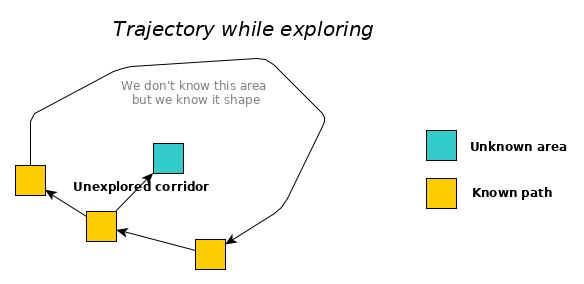
\includegraphics[scale=0.5]{ex_shape.jpg}\\
On peut alors savoir que cette aile est probablement sans issue (il faut pour cela tout de même supposer que le labyrinthe est euclidien). Cette déduction permettrait, dans le cas où la sortie est sur un bord, par exemple, de savoir qu'il ne vaut pas la peine d'explorer l'aile. On peut aussi en fonction de la taille maximale que peut avoir cette aile, si la sortie est dans une salle d'une certaine taille, déduire si oui ou non elle a la place de s'y trouver. Dans tous les cas, sans autres hypothèses on ne peut pas vraiment faire mieux.

\section{Conclusion}
Au final, on a bien réussit à extraire un réseau neuronal des équations de pseudo Navier-Stokes. Ce réseau de neurones fait même plus que ce qu'on attendait de lui car il est capable lui-même d'explorer et de réguler son exploration. Il résoud donc la plupart des labyrinthes de manière optimale et est bien meilleur que le Q-Learning classique en terme de nombre de pas dans le labyrinthe.

\section{Ouverture}
Je pense que le plus important dans ce travail n'est pas le fait de pouvoir mieux résoudre le problème du labyrinthe (cf Réflections sur le problème du labyrinthe). Le véritable intérêt et ce qui est vraiment innovant dedans c'est surtout d'avoir été capable d'extraire un réseau de neurones d'un lot de contraintes. Ce concept inédit permettrait de vraiment améliorer les possibilités du machine learning par la suite en permettant de travailler sur des modèles avec une convergence infiniment plus rapide, avec moins de données et avec une meilleure robustesse (on a éliminé plein de fonctions suite à la prise en compte des contraintes). Il est important que comprendre que pour faire des progrès en machine learning il y a 3 choses sur lesquelles on peut jouer : soit on fait les simulations plus vite donc on apprend plus vite. Soit on arrive à guider l'apprentissage afin de ne pas avoir à tout explorer (ce qui aboutit souvent à de bonnes solutions mais pas optimales), soit on arrive à garantir des performances sur la méthode employée (par exemple avoir une IA n'étant pas capable de blesser un humain). Ainsi même si on donne des contraintes et que l'on en fait un réseau de neurones, si elles ne balisent pas assez fortement le terrain, ce ne serra pas une grande avancée. Cependant si on arrivait à mieux développer ces techniques et si on arrivait à avoir une meilleure compréhension de cette forme d'apprentissage, alors on pourrait avoir de bien meilleurs résultats que les méthodes classiques. On pourrait alors par exemple, battre Google au niveau de la reconnaissance d'images car la quantité de données ne serrait plus un problème.\\
L'idéal serrait d'avoir une fonction qui étant donné un lot de contraintes, soit capable de produire un réseau de neurones particulier, spécifiquement fait pour résoudre le problème lié au lot de contraintes donné et qui renvoie NONE s'il n'en existe pas. Or ce genre de problème est typiquement non calculable (dépend de la formulation) et il y a donc du travail pour essayer de délimiter ce qui est calculable de ce qui ne l'est pas afin de voir si c'est une bonne direction à suivre pour des travaux futurs.

\bibliographystyle{}
\bibliography{biblio.bib}
\begin{comment}
\section{Annexes}
\subsection{Preuve (assez succinte) de l'indécidabilité}
\textbf{Données} : Un lot de contraintes (un ensemble d'équations supposé fini de la forme (\{$F_i$($X_i$) = 0\}$_{i\in\mathbb{N}}$ avec les $F_i$ des fonctions et $X_i$ des vecteurs de variables)). Ces équations portent sur une fonction f (celle que l'on cherche) mais peuvent aussi porter sur d'autre objets externes donc l'ensemble est noté E et est fini(comme d'autres fonctions, ce qui laisse beaucoup de possibilités).\\
\textbf{Expected Output} : Une fonction f$_{W,E}$ (avec W un vecteur de taille n$\in\mathbb{N}$) qui pour tout W de taille n
satisfait les contraintes.\\

On va considérer le problème de décision sous-jacent :\\
\textbf{Données} : Un lot de contraintes (un ensemble d'équations supposé fini de la forme (\{$F_i$($X_i$) = 0\}$_{i\in\mathbb{N}}$ avec les $F_i$ des fonctions et $X_i$ des vecteurs de variables)). Ces équations portent sur une fonction f (celle que l'on cherche) mais peuvent aussi porter sur d'autre objets externes dont l'ensemble est noté E et est fini.\\
\textbf{Problème} : Est-ce qu'il existe une fonction f$_{W,E}$ (avec W un vecteur de taille n$\in\mathbb{N}$) qui pour tout W de taille n satisfait ces contraintes ?\\

\textbf{Résumé:}\\
On va réduire le problème de l'arrêt : On va montrer que l'on peut coder toutes les formules logiques que l'on veut dans les contraintes puis on va coder une machine de Turing avec des portes logiques (je ne ferai pas le détail ici), enfin, pour une entrée donnée, si cette machine s'arrête sur cette entrée, on ajoute un symbole spécial (disons \#) au début de la bande. Enfin on ajoute un contrainte qui dit que ce symbole apparaîtra au bout d'un moment. On aura donc, une fonction f existe ssi la machine s'arrête sur l'entrée donnée. Donc le problème serra indécidable.\\\\
\textbf{Détail:}
Prenons une machine de Turing M ainsi que un mot d'entrée w. On construit M' qui, quand elle s'arrête écrit \# au début du ruban. On code M' en un nombre fini de formules logiques utilisant un nombre infini dénombrable de variables logiques.
Maintenant on va réécrire les formules logiques de la machine de Turing de la façon suivante, pour une formule f, on construit une formule $\widetilde f$ à travers le processus p (qui transforme f en $\widetilde f$):
\[f = a \wedge b \rightarrow \widetilde a.\widetilde b = \widetilde f \]
\[f = \lnot a \rightarrow 1-\widetilde a = \widetilde f\]
\[f = \forall x.g \rightarrow p(g) = \widetilde f\]
\[f = (a = b) \rightarrow (p(a) = p(b)) = \widetilde f\]
Les autres règles s'en déduisent.
La dernière règle utilise une notation curryfiée, on considère que 
\[(h:x\rightarrow0) = 0\]
Ainsi il faut comprendre : si $\forall x.g(x)$ (est vraie), alors $g$ (est vraie) et on transforme g récursivement. Ensuite, pour le stockage des variables, vu que l'on a un ensemble dénombrable de variables, on peut utiliser une fonction Memory : 
\[Memory : \mathbb{N} \rightarrow \{0,1\}\cup MemEns\]
avec MemEns étant l'ensemble des fonctions de $\mathbb{N}$ dans $\{0,1\}\cup \text{MemEns}$ (on peut un peut voir Memory comme un arbre : soit un entier donne une feuille et donc une valeur entre 0 et 1, soit elle donne un noeud : une autre fonction Memory). Ainsi quand on voit une variable logique pendant la transformation par p $a_{X}$ avec X un vecteur ayant potentiellement plusieurs composantes, on va la remplacer par Memory(name(a))[X], avec name un fonction qui étiquette chaque symbole de variable (ne peut apparaître que en nombre fini) par un entier différent (par exemple, $a_X$ devient 1, $b_Y$ devient 2, ... sans distinction de leurs indices). Ainsi, la fonction Memory principale n'étiquette que les symboles, puis on applique récursivement le procédé suivant :
\[X = (x1,x2,...xn)\]
\[X2 = (x2,...,xn)\]
\[Memory(name(a))[X,Y,...] = 
\begin{cases}
	Memory(name(a))[x1,X2,Y,...] & \text{x1 vecteur} \\
	\begin{cases}
		Memory(name(a))(x1)[X2,Y,...] & X2 \neq []\\
		Memory(name(a))(x1)[Y,...] & X2 = []
	\end{cases} & \text{sinon}
\end{cases}
\]
et 
\[Memory(name(a))(x1)...(zn)[] = Memory(name(a)(x1)...(zn)\]
Quand la stack d'arbres est vide , on a la valeur de notre variable qui serra dans la contrainte. Ainsi pour chaque variables logique qui apparaît dans les formules logiques, on a un chemin dans Memory qui code cette variable dans [0,1]. De plus, chaque contrainte finira par = 1 (vraie). On va encore rajouter une contrainte : 
\[p(\exists n.Bande(n)(0)=\#)\]
avec Bande(t)(x) la fonction qui à un instant t, associe le caractère codé en position x sur la bande.
On peut donc bien transformer ces formules booléennes du 1er ordre qui sont en nombre fini en contraintes puis donner ces contraintes à notre fonction dont on veut démontrer la non calculabilité.\\
On a alors : la fonction f existe ssi la machine termine. Donc indécidable.
\end{comment}
\newpage
\subsection{pNSNeuron}
\indent\indent\indent\indent\rotatebox{270}{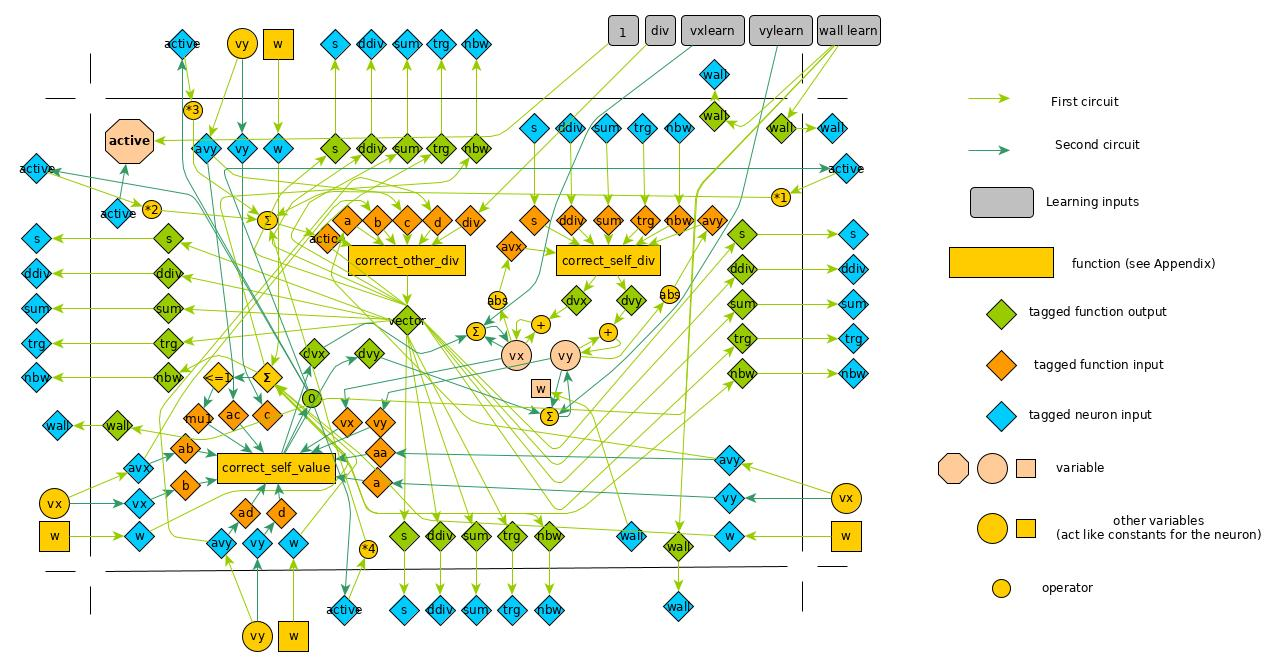
\includegraphics[scale=0.48]{pNSNeu.jpg}}\\

\newpage
\paragraph{Correct Self Div Organelle}-\\
\rotatebox{270}{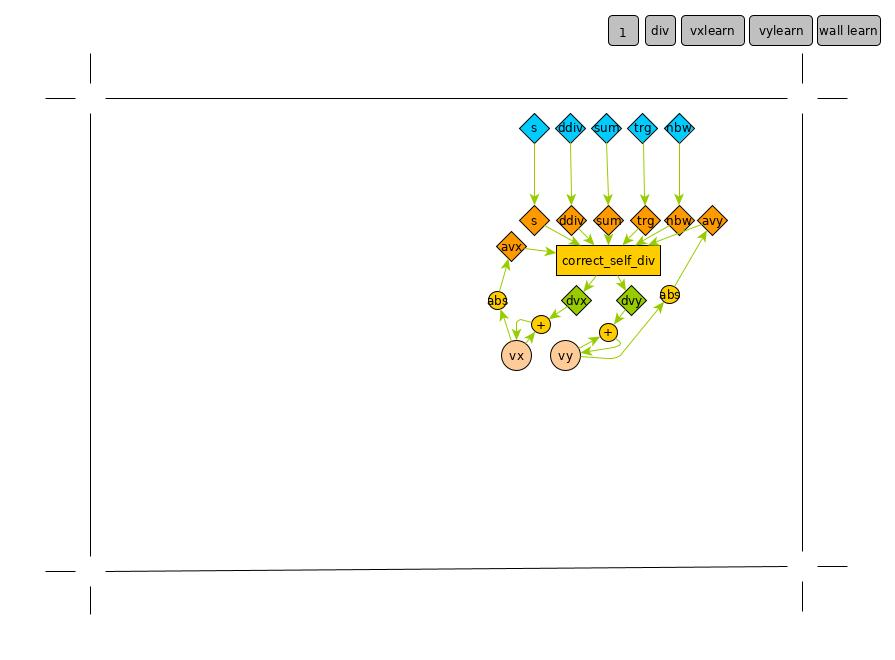
\includegraphics[scale=0.60]{correct_self_div_organelle.jpg}}\\

\newpage
\paragraph{Correct Other Div Organelle}-\\
\rotatebox{270}{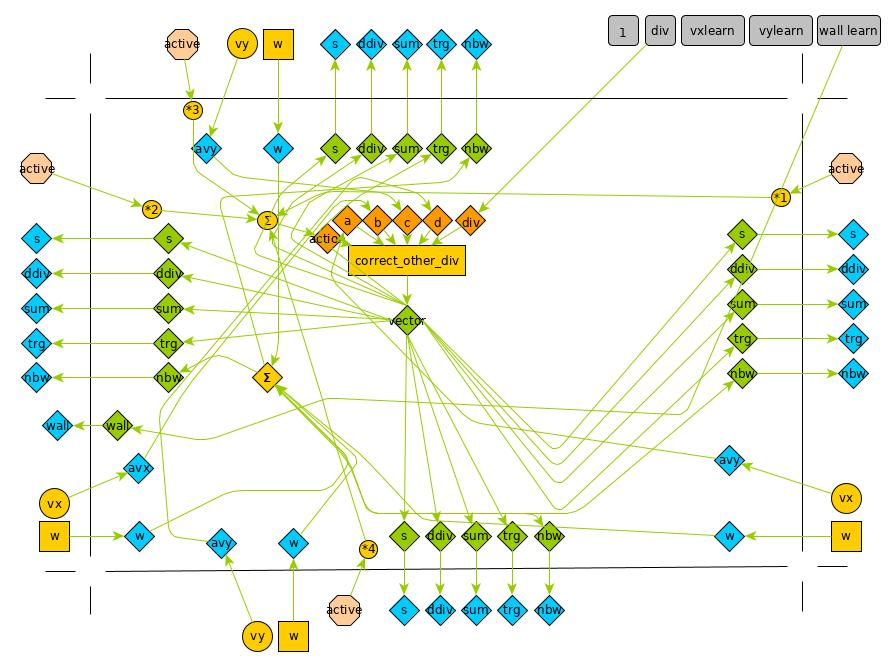
\includegraphics[scale=0.6]{correct_other_div_organelle.jpg}}\\

\newpage
\paragraph{Correct Self Value Organelle}-\\
\rotatebox{270}{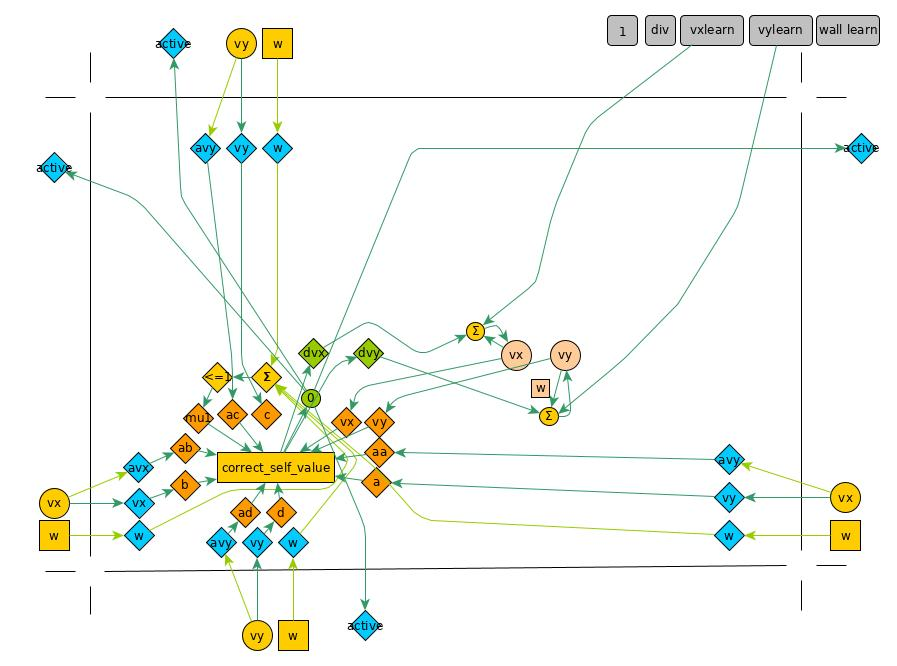
\includegraphics[scale=0.6]{correct_self_value_organelle.jpg}}\\

\newpage
\paragraph{Active Organelle}-\\
\rotatebox{270}{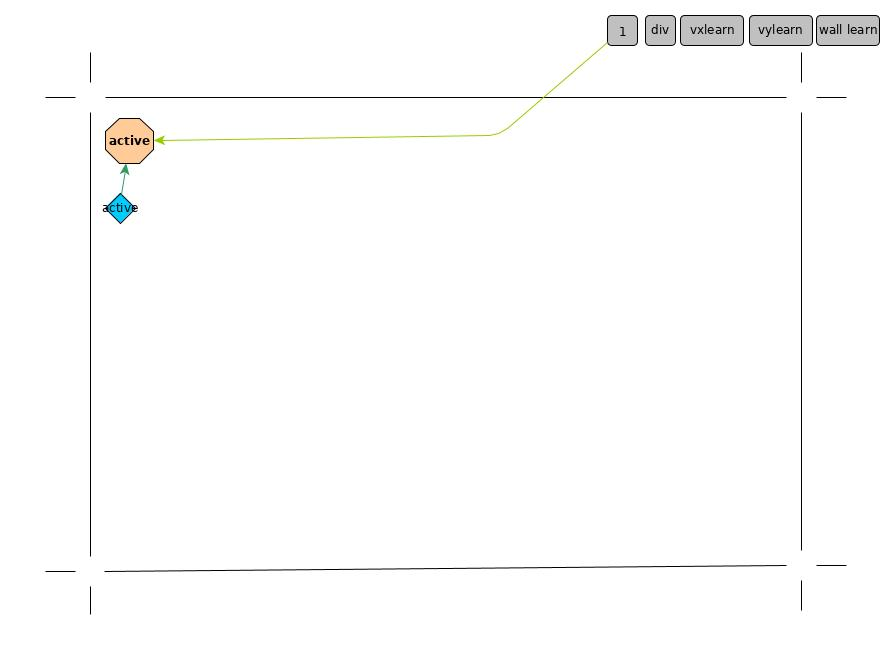
\includegraphics[scale=0.6]{active_organelle.jpg}}\\

\newpage
\paragraph{Correct Other Wall Organelle}-\\
\rotatebox{270}{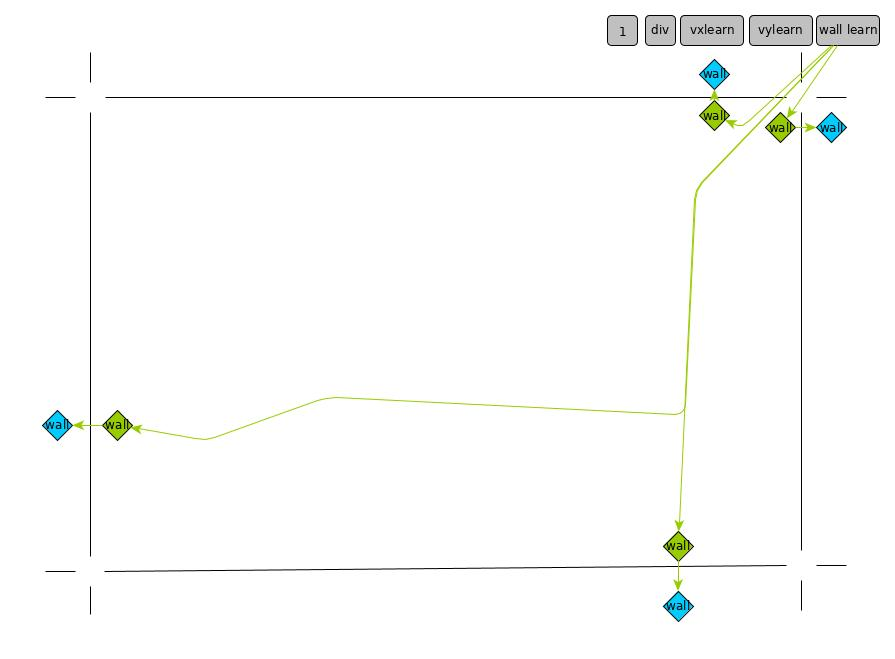
\includegraphics[scale=0.6]{correct_other_wall_organelle.jpg}}\\

\newpage
\paragraph{Correct Self Wall Organelle}-\\
\rotatebox{270}{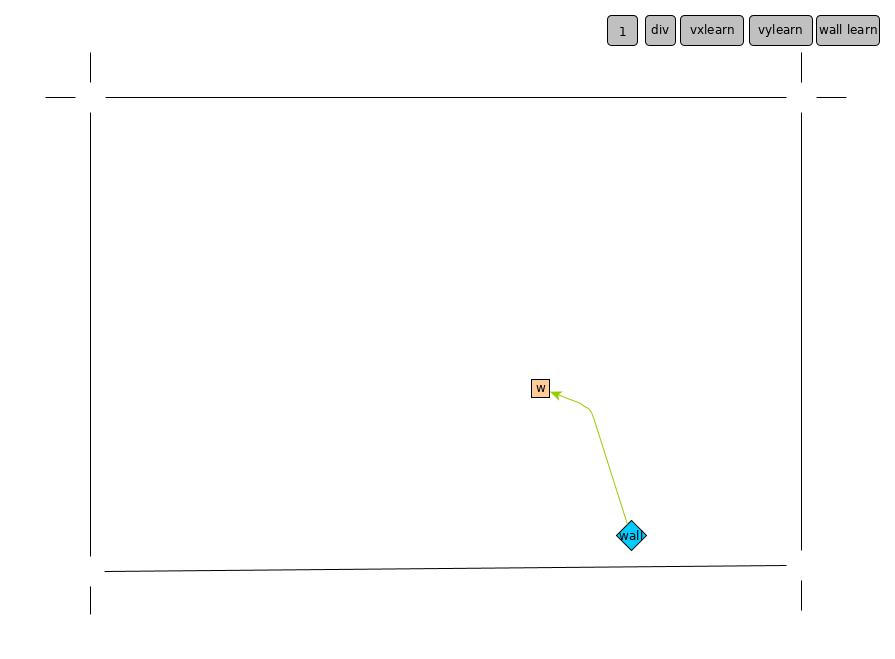
\includegraphics[scale=0.6]{correct_self_wall_organelle.jpg}}\\

\newpage
\subsection{Functions}
\begin{algorithm}
\caption{correct\_self\_div}
\begin{algorithmic}
\REQUIRE{s,ddiv,sum,nbw,trg,avx,avy}
\IF{$sum == 0$}
\IF{$trg == 1$}
\STATE dvx $\leftarrow$ s*ddiv/nbw
\STATE dvy $\leftarrow$ 0
\ELSE
\STATE dvx $\leftarrow$ 0
\STATE dvy $\leftarrow$ s*ddiv/nbw
\ENDIF
\ELSE
\IF{$trg == 1$}
\STATE dvx $\leftarrow$ s*ddiv*avx/sum
\STATE dvy $\leftarrow$ 0
\ELSE
\STATE dvx $\leftarrow$ 0
\STATE dvy $\leftarrow$ s*ddiv*avy/sum
\ENDIF
\ENDIF
\RETURN dvx,dvy
\end{algorithmic}
\end{algorithm}

\begin{algorithm}
\caption{correct\_other\_div}
\begin{algorithmic}
\REQUIRE{a,b,c,d,active}
\STATE ddiv $\leftarrow$ a-b+c-d
\STATE s $\leftarrow$ a+b
\STATE sum $\leftarrow$ 0
\IF{$active\neq0$}
\STATE sum $\leftarrow$ sum + abs(a)
\ENDIF
\IF{$active\neq1$}
\STATE sum $\leftarrow$ sum + abs(b)
\ENDIF
\IF{$active\neq2$}
\STATE sum $\leftarrow$ sum + abs(c)
\ENDIF
\IF{$active\neq3$}
\STATE sum $\leftarrow$ sum + abs(d)
\ENDIF
\STATE nbw $\leftarrow$ wa+wb+wc+wd
\STATE top,bottom $\leftarrow$ (s,ddiv,sum,1)
\STATE left,right $\leftarrow$ (s,ddiv,sum,0)
\STATE vector $\leftarrow$ \{"top":top,"left":left,"bottom":bottom,"right":right\}
\RETURN vector
\end{algorithmic}
\end{algorithm}

\begin{algorithm}
\caption{correct\_self\_value}
\begin{algorithmic}
\REQUIRE{a,b,c,d,svx,svy,aa,ab,ac,ad,vx,vy}
\STATE avex $\leftarrow$ (a+b)/2
\STATE avey $\leftarrow$ (c+d)/2
\STATE sv $\leftarrow$ sv(vx)*sv(vy)
\STATE dev $\leftarrow$ mu*sv*(((ac*vy$<$0)+(ad*vy$<$0))*abs(vy)/2-((aa*vx$<$0)+(ab*vx$<$0))*abs(vx)/2)
\STATE dvx $\leftarrow$ avex+dev
\STATE dvy $\leftarrow$ avey-dev
\RETURN dvx,dvy
\end{algorithmic}
\end{algorithm}
\newpage
\section{Comparaison pNSNeurons / Q-Learning tabulaire}
\subsection{maze 1}
\indent\indent\indent\indent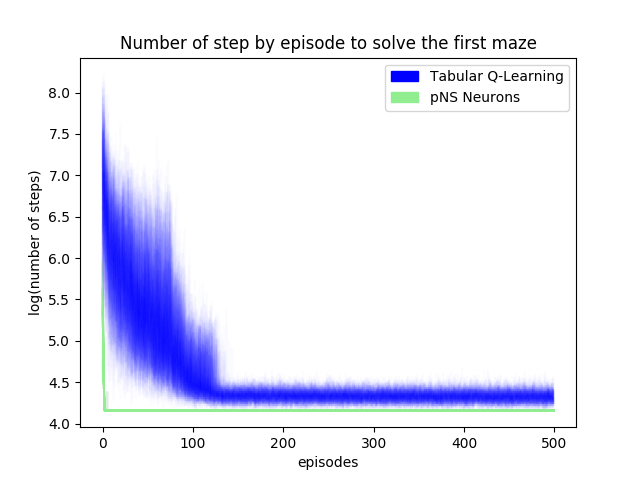
\includegraphics[scale=0.48]{Figure_log_final.png}\\

\subsection{maze 2}
\indent\indent\indent\indent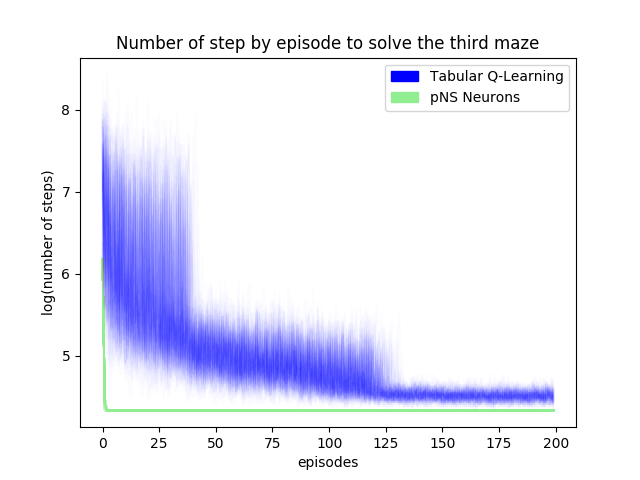
\includegraphics[scale=0.48]{Figure_log_final2.png}\\

\subsection{maze 3}
\indent\indent\indent\indent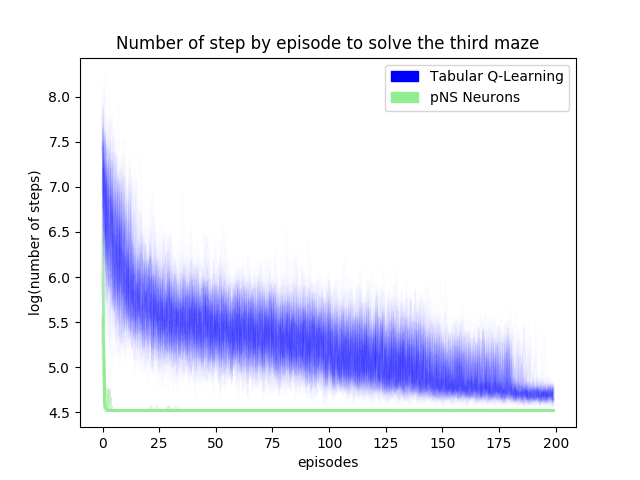
\includegraphics[scale=0.48]{Figure_log_final3.png}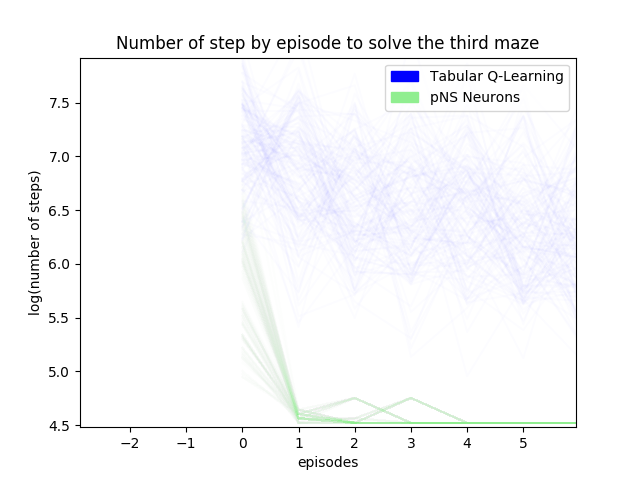
\includegraphics[scale=0.48]{Figure_log_beg3.png}\\

\end{document}